% !TeX program = xelatex
\documentclass{article}
\usepackage[paperwidth=6.75in,paperheight=2.45in,margin=.08in]{geometry}
\usepackage{tikz}
\usepackage{fontspec}
\setmainfont{texgyreheros-regular.otf}
\setsansfont{texgyreheros-regular.otf}
\usetikzlibrary{positioning,arrows.meta}
\renewcommand{\familydefault}{\sfdefault}
\pagestyle{empty}
\begin{document}
\noindent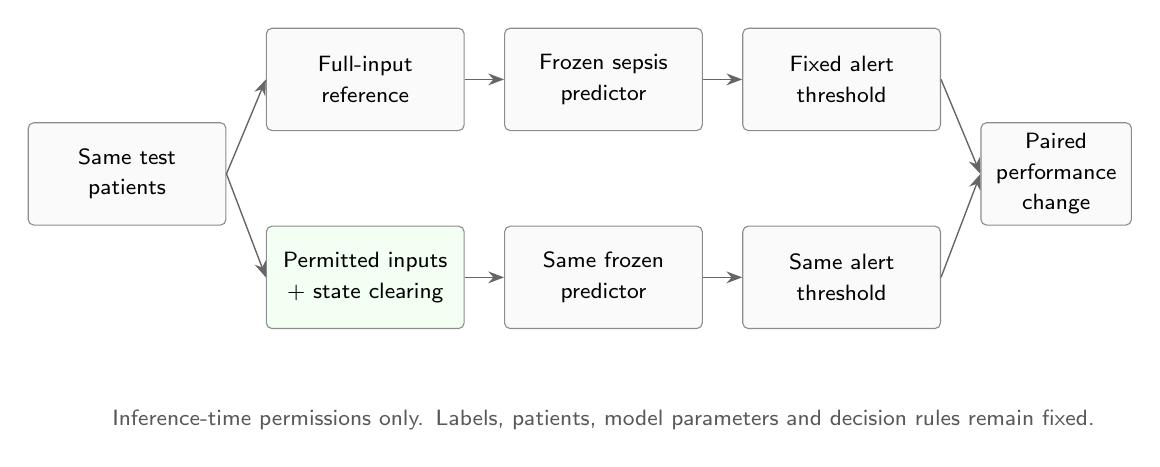
\begin{tikzpicture}[font=\sffamily\fontsize{8}{11}\selectfont,node distance=6mm and 5mm,
block/.style={draw=black!45,rounded corners=2pt,fill=black!2,text width=23mm,minimum height=13mm,align=center,inner sep=3pt},
flow/.style={-{Stealth[length=2mm]},draw=black!60,line width=.5pt}]
\node[block] (patients) {Same test\\patients};
\node[block,right=of patients,yshift=12mm] (full) {Full-input\\reference};
\node[block,below=12mm of full,fill=green!5!white] (mask) {Permitted inputs\\+ state clearing};
\node[block,right=of full] (model) {Frozen sepsis\\predictor};
\node[block,right=of mask] (restricted) {Same frozen\\predictor};
\node[block,right=of model] (policy) {Fixed alert\\threshold};
\node[block,right=of restricted] (samepolicy) {Same alert\\threshold};
\node[block,right=of policy,yshift=-12mm,text width=17mm] (delta) {Paired\\performance\\change};
\draw[flow] (patients.east) -- (full.west);
\draw[flow] (patients.east) -- (mask.west);
\draw[flow] (full) -- (model);\draw[flow] (mask) -- (restricted);
\draw[flow] (model) -- (policy);\draw[flow] (restricted) -- (samepolicy);
\draw[flow] (policy.east) -- (delta.west);\draw[flow] (samepolicy.east) -- (delta.west);
\node[below=9mm of restricted,text width=125mm,align=center,font=\sffamily\fontsize{8}{11}\selectfont,text=black!65] {Inference-time permissions only. Labels, patients, model parameters and decision rules remain fixed.};
\end{tikzpicture}
\end{document}
